\section{Machine Learning Framework}


RL owes its success partly to a strong function approximator, deep neural networks. Where tabular Q-function only solved games like tic-tac-toe, neural networks integration to Q-function scales to high dimensional complex tasks like Atari games \cite{Mnih}. The growing success of neural networks inspired large companies like Google and Facebook to start their own open-source machine learning frameworks. Among those projects, Tensorflow, Keras, and PyTorch are the most popular ones \cite{Tensoflow} \cite{Keras} \cite{PyTorch}. 

Granted that we decided to work with Tensorflow and Keras on different parts of the project, it is worth mentioning that PyTorch is becoming dominant in research \cite{Horace}. In figure \ref{fig:ptvstf} demonstrates how Pytorch has risen steeply in terms of mentions in the major conferences. It achieved a staggering comeback from a maximum of \(6\%\) mentions to \(78.72\%\) mentions in three years.  

\begin{figure}[htbp] 
    \centering
    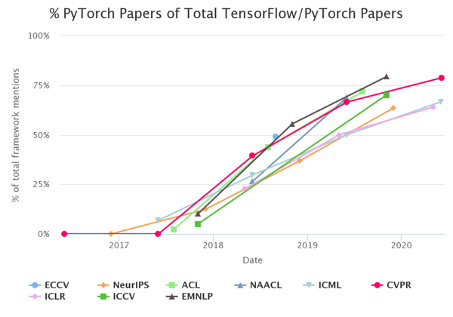
\includegraphics[width=0.7\textwidth]{figures/tfvspytorch}
    \caption{PyTorch and Tensorflow comparison based on the mentions in major machine learning conferences \cite{Horace}}
    \label{fig:ptvstf}
\end{figure}


According to the researchers, PyTorch's success is due to simplicity, great API, and performance. Even Tensorflow, in its last edition Eager, delivered a similar API to PyTorch. Though, there have been reports about the weaknesses of Eager in performance and memory. In short, it is unlikely that Tensorflow recovers and catches PyTorch anytime soon.

In conclusion, it is also possible to see the transition from Tensorflow to Pytorch in the RL community. Stable Baselines released the PyTorch version of Baselines algorithms in May 2020 \cite{stable-baselines3}. OpenAI Spinningup, an educational incentive for RL teaching from OpenAI, has moved to PyTorch in February 2020. Furthermore, they now host the master branch with PyTorch implementation \cite{SpinningUp2018}.

 